L'acceleratore utilizzato è un acceleratore per ricerca sulla flash di fisica medica. È l'unico al mondo che permette di raggiungere alti dosaggi mantenendo l'indipendenza dei parametri del fascio. La struttura del fascio e le varie quantita che si usano per descriverlo sono riportate in figure \ref{fig:}.



\begin{figure}
    \centering
    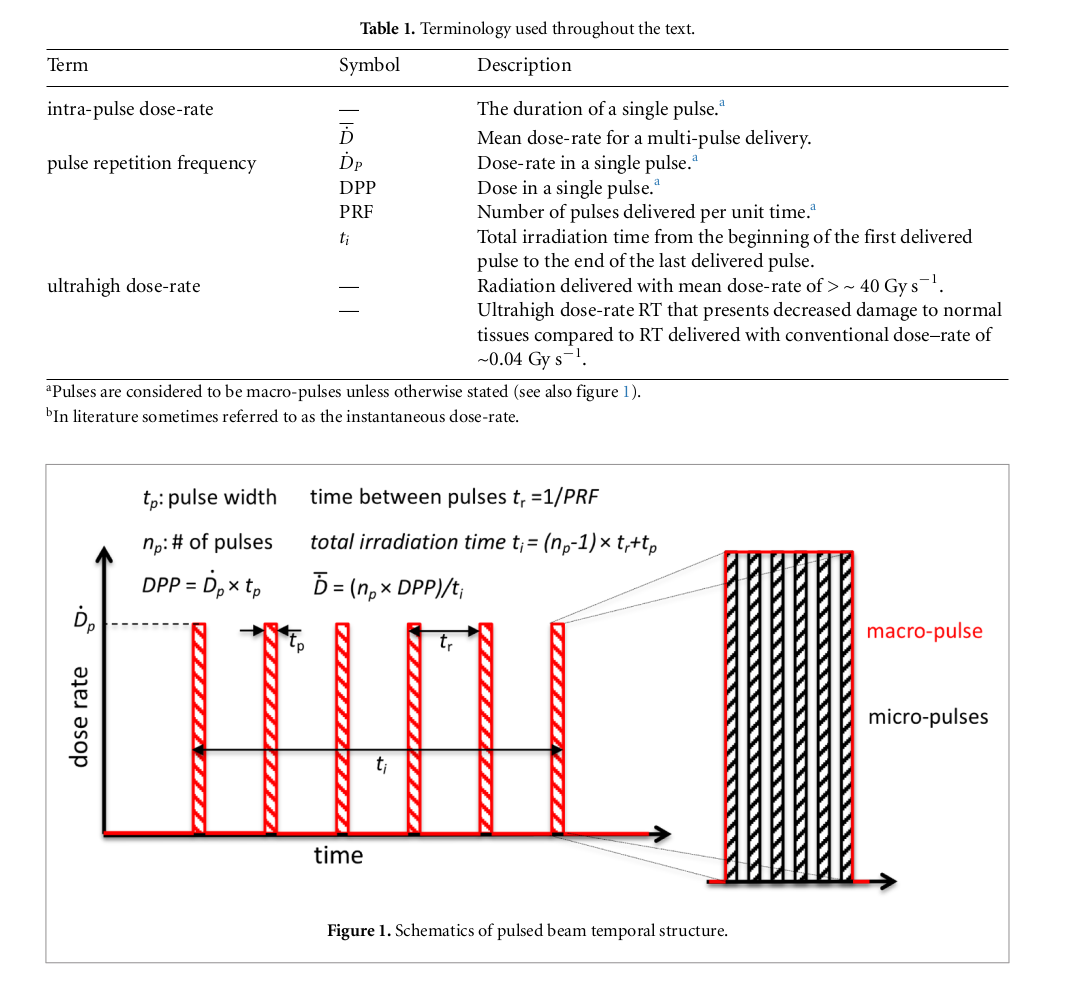
\includegraphics[width=.98\linewidth]{figures/test_beam/dose_param.png}
    \caption{}
    \label{fig:}
 \end{figure}


 \begin{equation}
    R[Hz/cm^2] = \frac{DPP[Gy]}{1.6 \;10^{10} S[g/cm^2]}
 \end{equation}
 where S is the stopping power in water, \SI{2.17}{g/cm\squared}


 Possibilità di integrare carica sul pixel: due elettroni consecutivi su un pixel ogni quanto arrivano?

Vogliamo sfruttare l'analog pile up, per fare questo dobbiamo fare attenzione a non finire nel digital pile up
Devi avere che il tot dell'elettrone (cioè MIP) è maggiore del deltat medio; in questo caso potresti riuscire ad integrare carica.

